  \section[Docker]{Vue d'ensemble}

  \subsection[Docker]{Docker : les concepts}

  \begin{frame}
    \frametitle{Un ensemble de composants}
    \begin{itemize}
      \item Layers
      \item Stockage
      \begin{itemize}
          \item Volumes \pause
      \end{itemize}
      \item Réseau
      \begin{itemize}
          \item Ports \pause
          \item Links \pause
      \end{itemize}
    \end{itemize}
  \end{frame}

  \begin{frame}
    \frametitle{Layers : une image}
    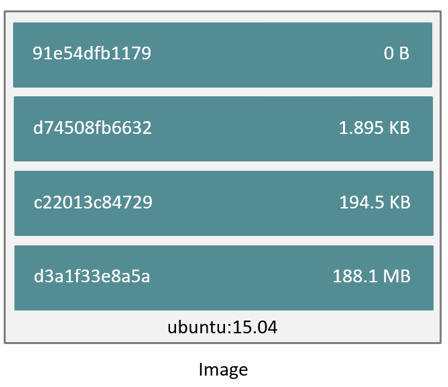
\includegraphics[height=200px]{images/docker/image-layers.jpg}
  \end{frame}

  \begin{frame}
    \frametitle{Layers : un conteneur}
    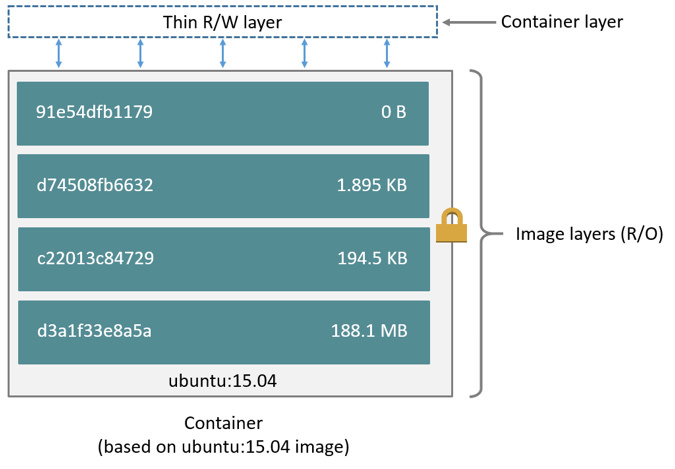
\includegraphics[height=200px]{images/docker/container-layers.jpg}
  \end{frame}

 \begin{frame}
    \frametitle{Layers : plusieurs conteneurs}
    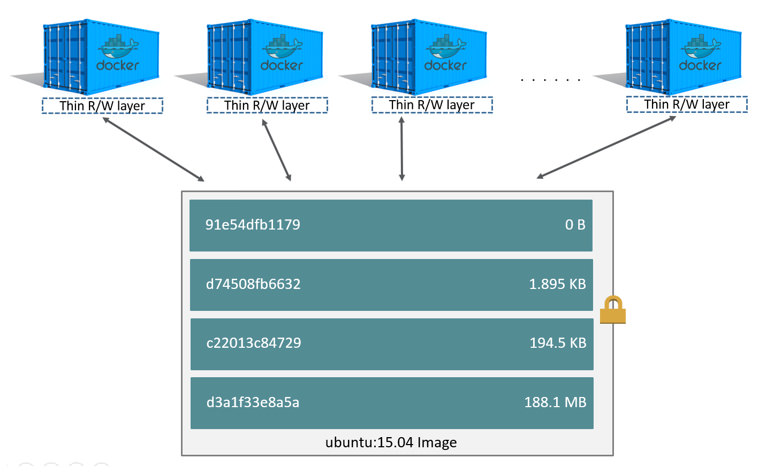
\includegraphics[height=200px]{images/docker/sharing-layers.jpg}
  \end{frame}

 \begin{frame}
    \frametitle{Layers : Répétition des layers}
    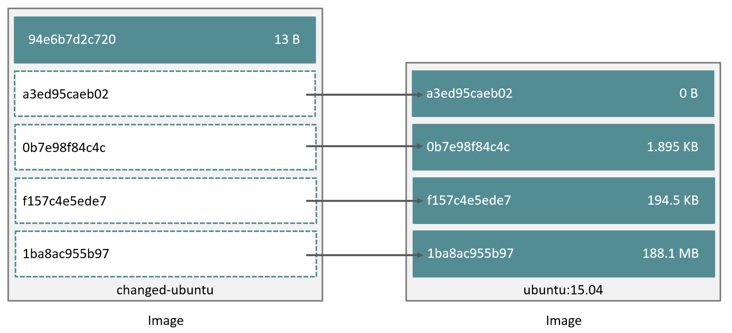
\includegraphics[height=200px]{images/docker/saving-space.jpg}
  \end{frame}

  \begin{frame}
    \frametitle{Stockage : volumes}
    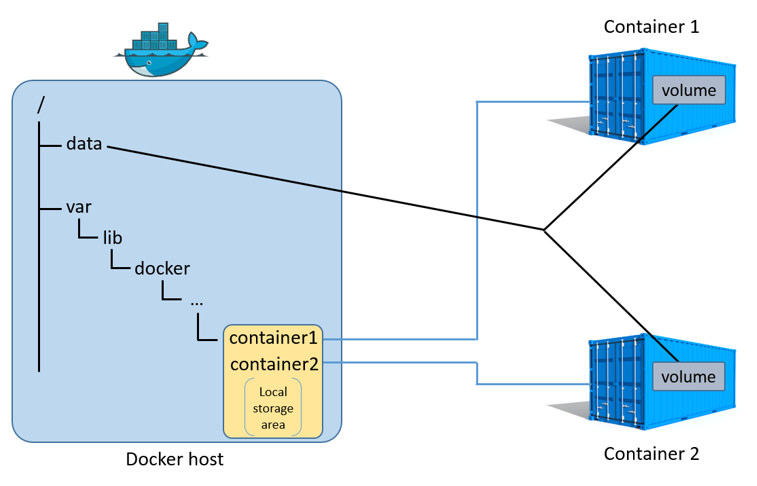
\includegraphics[height=200px]{images/docker/shared-volume.jpg}
  \end{frame}

  \begin{frame}
    \frametitle{Réseau, link et ports}
    A la base, pas grand chose...
\begin{verbatim}
NETWORK ID          NAME                DRIVER
42f7f9558b7a        bridge              bridge
6ebf7b150515        none                null
0509391a1fbd        host                host
\end{verbatim}
  \end{frame}
